\documentclass[12pt,a4paper]{article}

\usepackage[utf8]{inputenc} \usepackage[T1]{fontenc} \usepackage{graphicx}
\usepackage{longtable} \usepackage{tabularx} \usepackage{float}
\usepackage{wrapfig} \usepackage{soul} \usepackage{amssymb}
\usepackage{hyperref} \usepackage{caption} \usepackage{subcaption}
\usepackage{pdfpages} \usepackage{sidecap}


\parindent 0in \usepackage[spanish]{babel}
\setlength{\parskip}{0.5\baselineskip} \usepackage{fullpage}
\usepackage{multirow} \usepackage{multicol} \usepackage{framed}
\usepackage{listings} \usepackage{enumerate}

\usepackage{appendix} \usepackage{setspace} \usepackage{amsmath}


%% DEFINICIONES
\newcommand{\TODO}[1]{{\huge \color{red} \textbf{TODO: }#1 }}
\newcommand{\todo}[1]{{\large \color{red} \textbf{TODO: }#1 }}


\title{Práctica 2. \\ Geometría computacional} 

\author{Luis María Costero Valero (lcostero@ucm.es)\\ Jesús Doménech
  Arellano (jdomenec@ucm.es) \\ Jennifer Hernández Bécares (jennhern@ucm.es)}
\date{Marzo 2015}

\begin{document}
\maketitle
\decimalpoint

En esta práctica entregamos dos versiones del código, la primera en el
archivo \texttt{P2.py} y la segunda en \texttt{P2\_interactivo.py}. La diferencia es que la
segunda versión permite meter las condiciones iniciales de la
geodésica pinchando en la ventana gráfica. Dado que el código se complica,
entregamos la versión sin esta mejora para facilitar la corrección de
la práctica.

\begin{enumerate}
\item Dado el toro de revolución usual, dibújese sobre el mismo una
  geodésica cuya traza sea uno de los dos círculos generadores.\\
  Dibujamos el toro con $r = 2.0$ y $a = 5.0$ \\
  Para el círculo generador tomamos de condiciones iniciales:
  \begin{itemize}
  \item $(u_0, v_0) = (0, 0)$
  \item $(u'_0, v'_0) = (0, 1)$
  \end{itemize}

  \begin{center}
    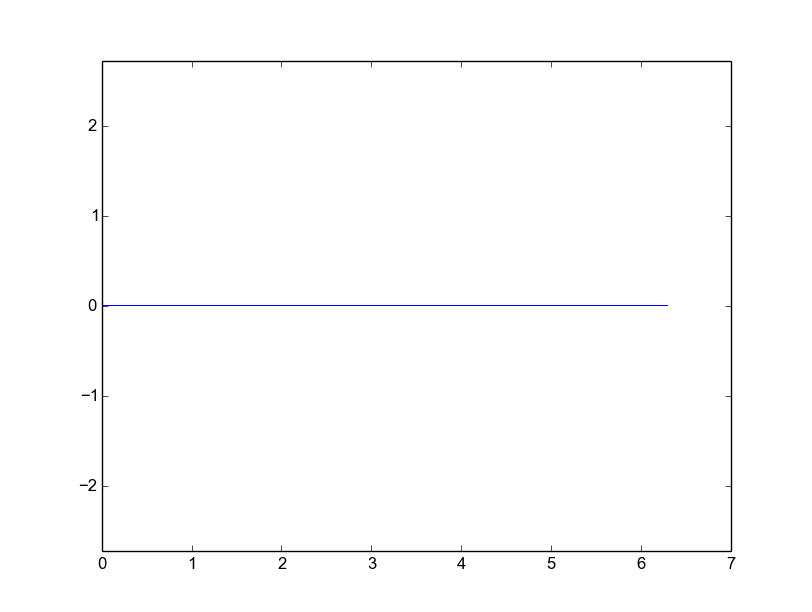
\includegraphics[width=0.4\textwidth]{./img/circulo1_trace.png}
    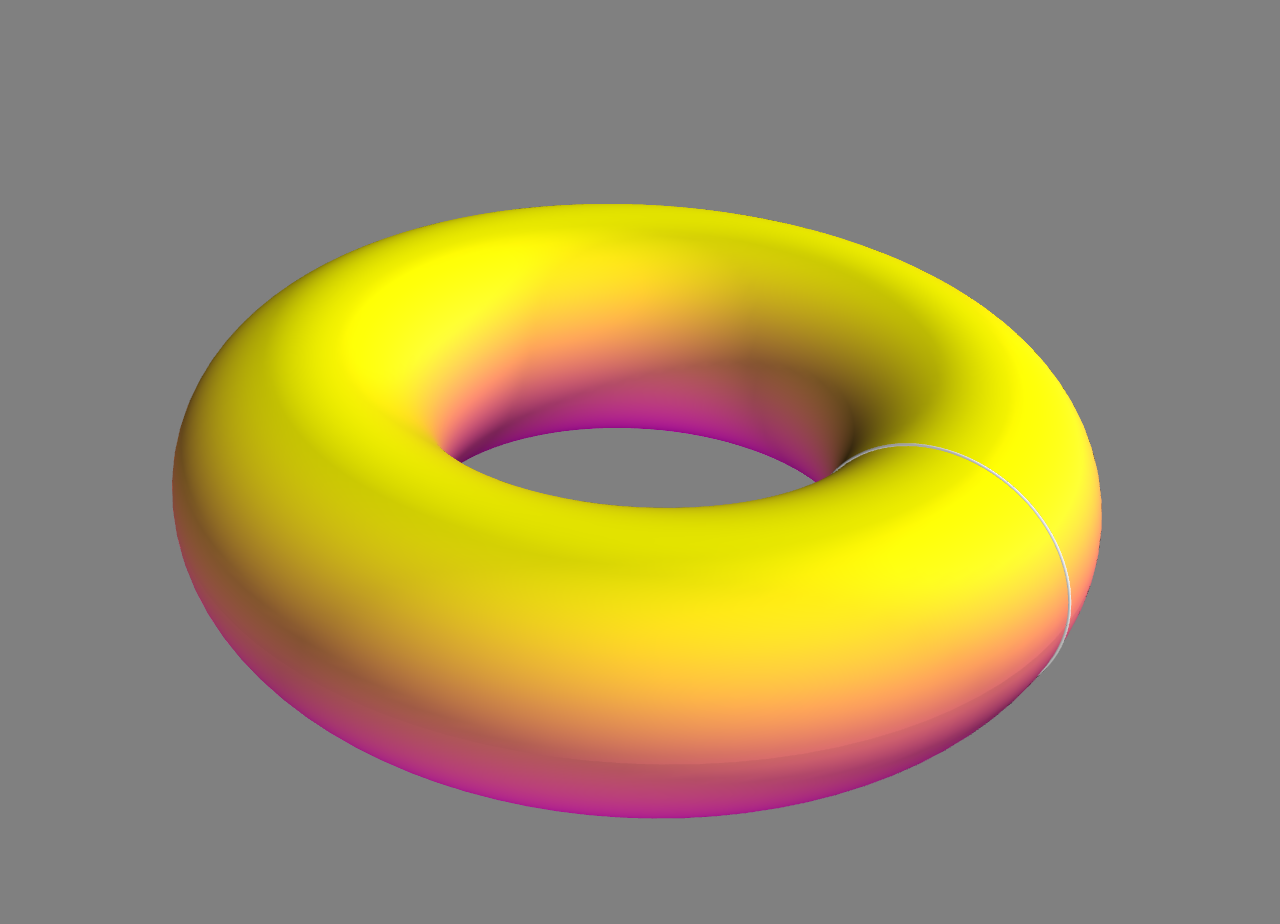
\includegraphics[width=0.4\textwidth]{./img/circulo1_surface.png}
  \end{center}

  El otro cículo generador se obtiene al establecer las derivadas iniciales
  como\\ $(u'_0, v'_0) = (1, 0)$
\newpage{}
\item Dibújese sobre el toro una geodésica periódica. Dibújese sobre
  el toro una geodésica no periódica. Opcional: ¿Sabrías obtenener una
  geodésica que sea densa sobre todo el toro?
  \begin{enumerate}
  \item Periódica: 
    \begin{center}
      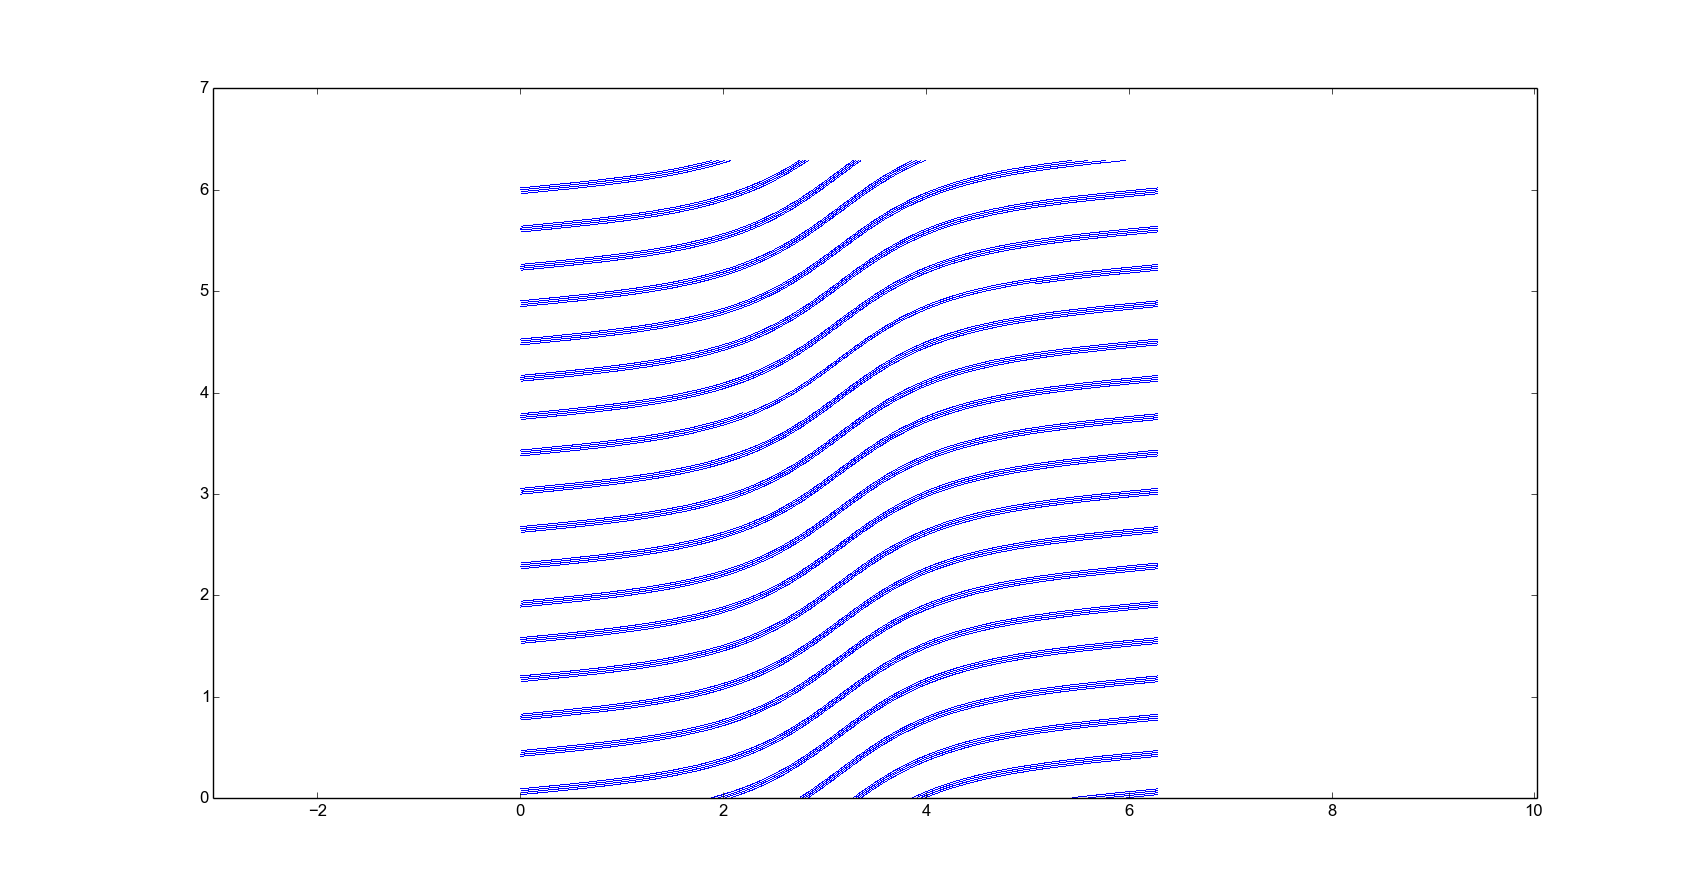
\includegraphics[width=0.4\textwidth]{./img/periodica_trace.png}
      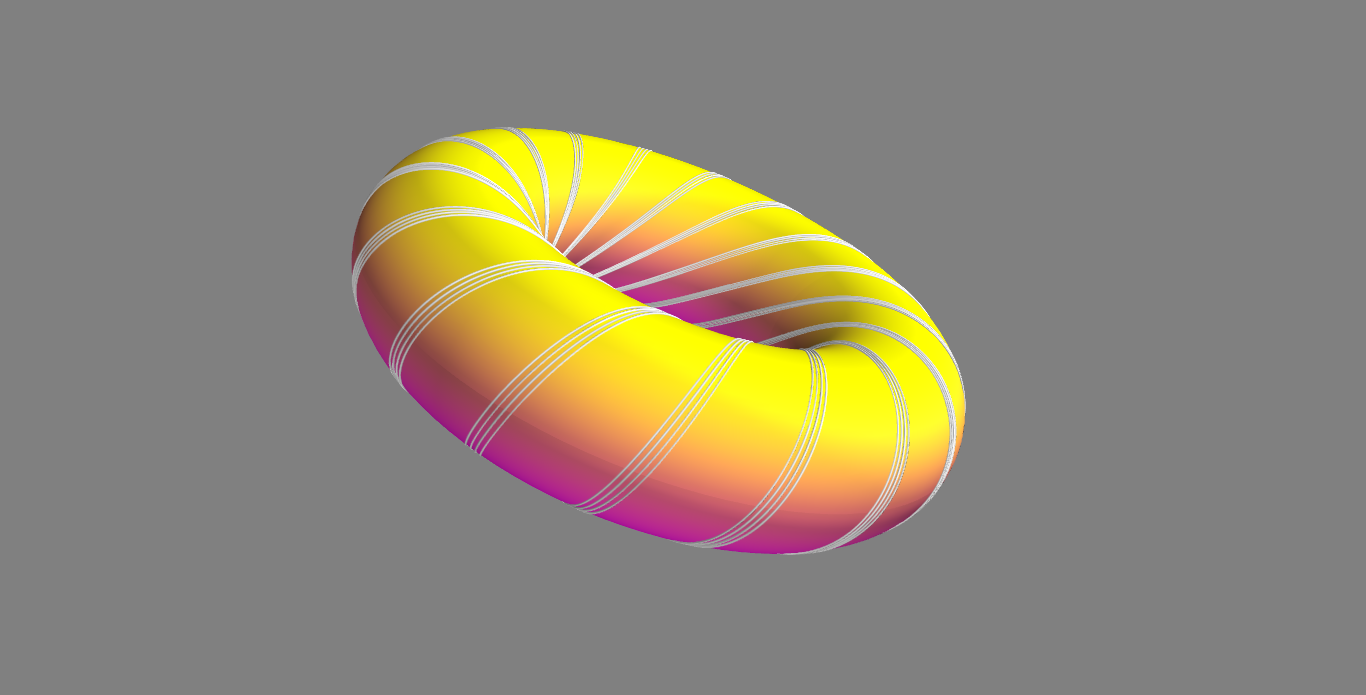
\includegraphics[width=0.4\textwidth]{./img/periodica_surface.png}
    \end{center}
  \item No periódica:
    \begin{itemize}
    \item $(u_0, v_0) = (\pi, 0)$
    \item $(u'_0, v'_0) = (1, \pi) $
      \begin{center}
        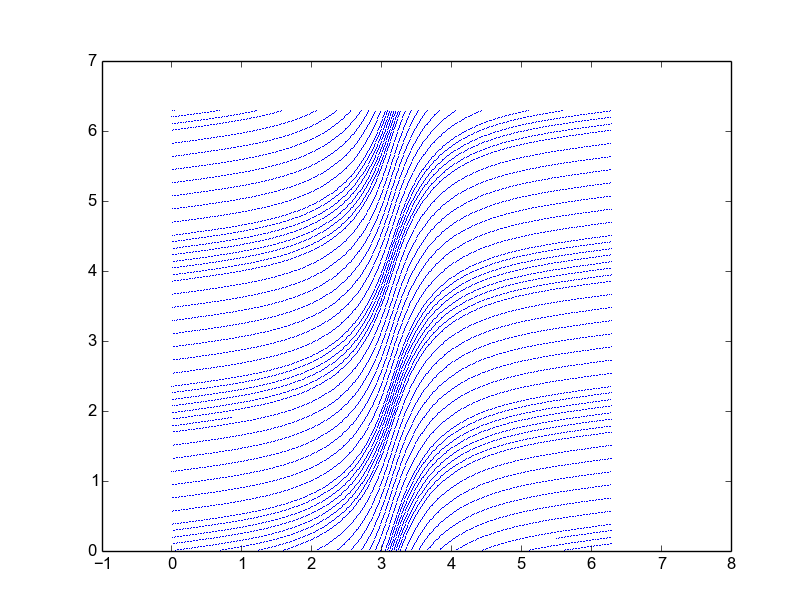
\includegraphics[width=0.4\textwidth]{./img/noperiodico_trace.png}
        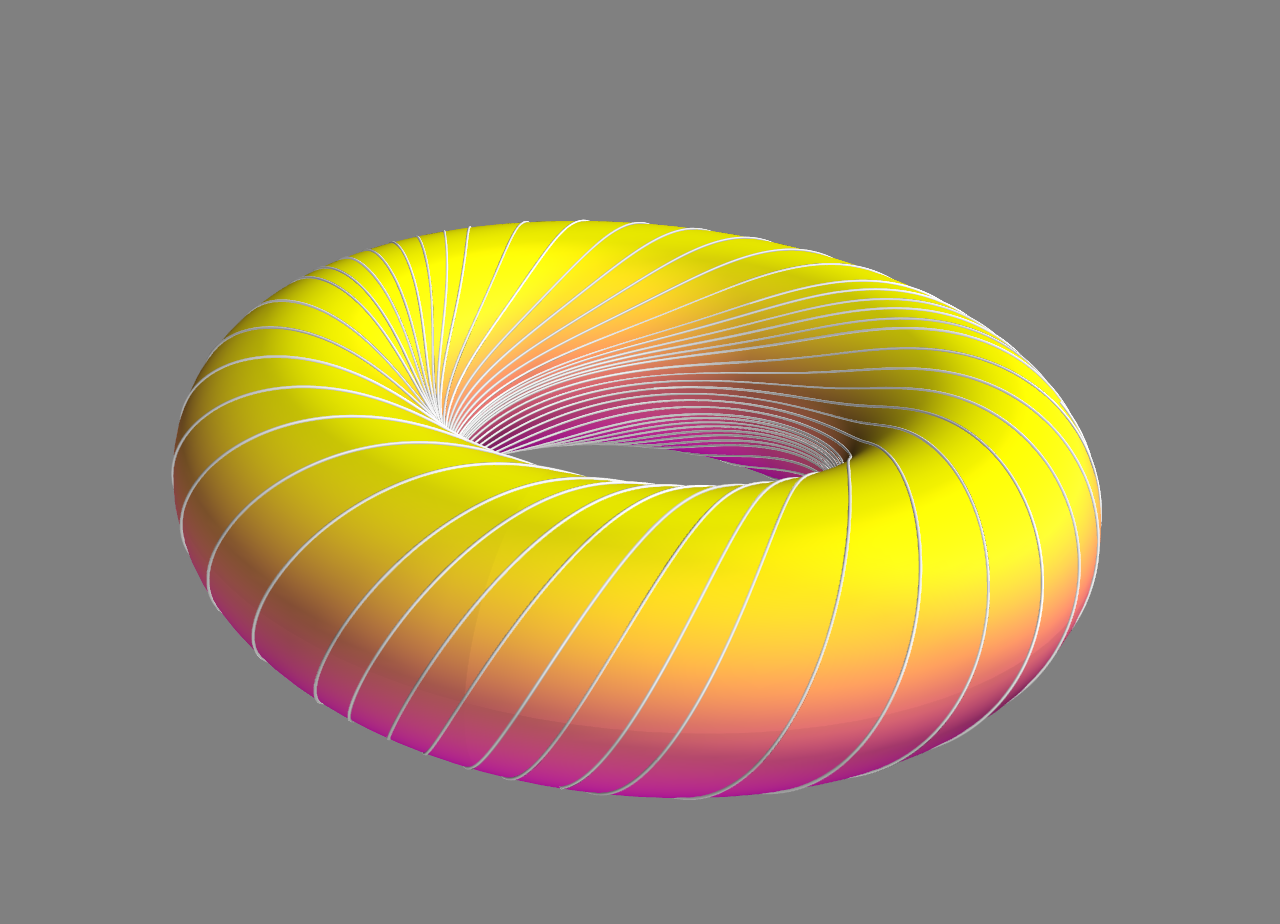
\includegraphics[width=0.4\textwidth]{./img/noperiodico_surface.png}
      \end{center}

    \end{itemize}
  \item Densa: Se propone las siguientes condiciones iniciales sobre una
    pendiente irracional para obtener una geodésica densa:
    \begin{itemize}
    \item $(u_0, v_0) = (\pi, 0) $
    \item $(u'_0, v'_0) = (1, 15\pi) $
      \begin{center}
        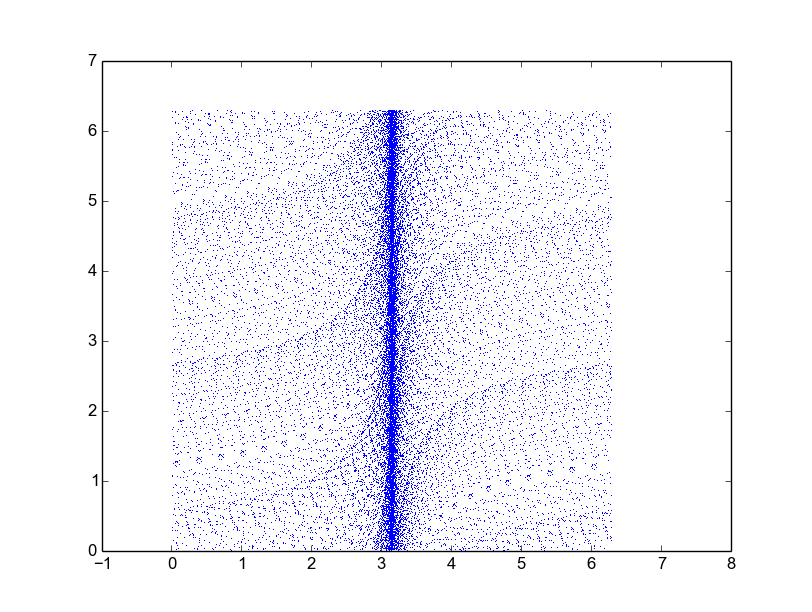
\includegraphics[width=0.4\textwidth]{./img/denso_trace.png}
        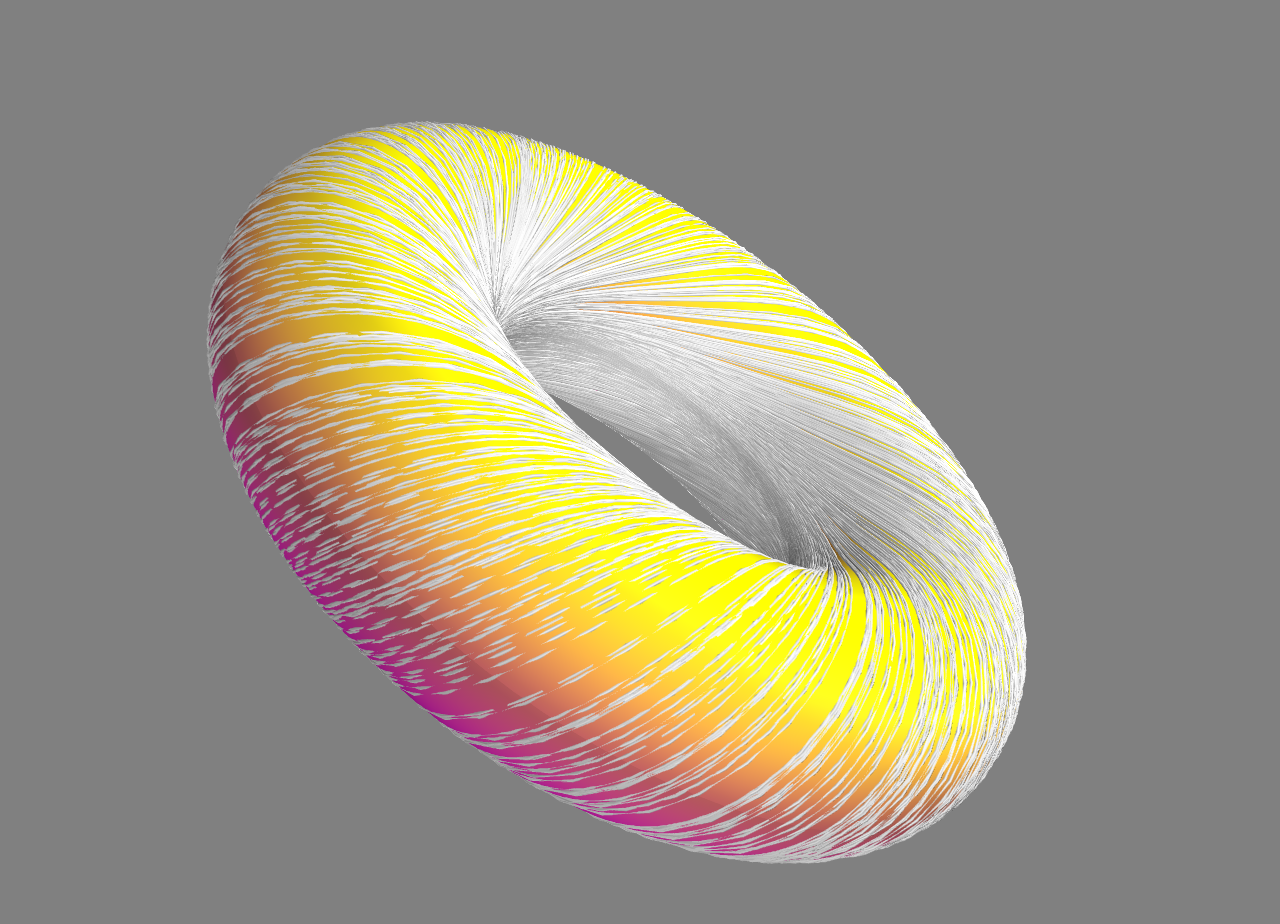
\includegraphics[width=0.4\textwidth]{./img/denso_surface.png}
      \end{center}
    \end{itemize}
  \end{enumerate}
\newpage{}
\item Modelo de plano hiperbólico dado por el semiplano de
  Poincaré. Considérese la primera forma fundamental en el semiplano
  $v>0$ dada por $E = G = \frac{1}{v^{2}}$ y $G = 0$. Dibújense sus
  geodésicas. Opcional: ¿Sabrías encontrar expresiones analíticas de
  las mismas?
  \begin{center}
    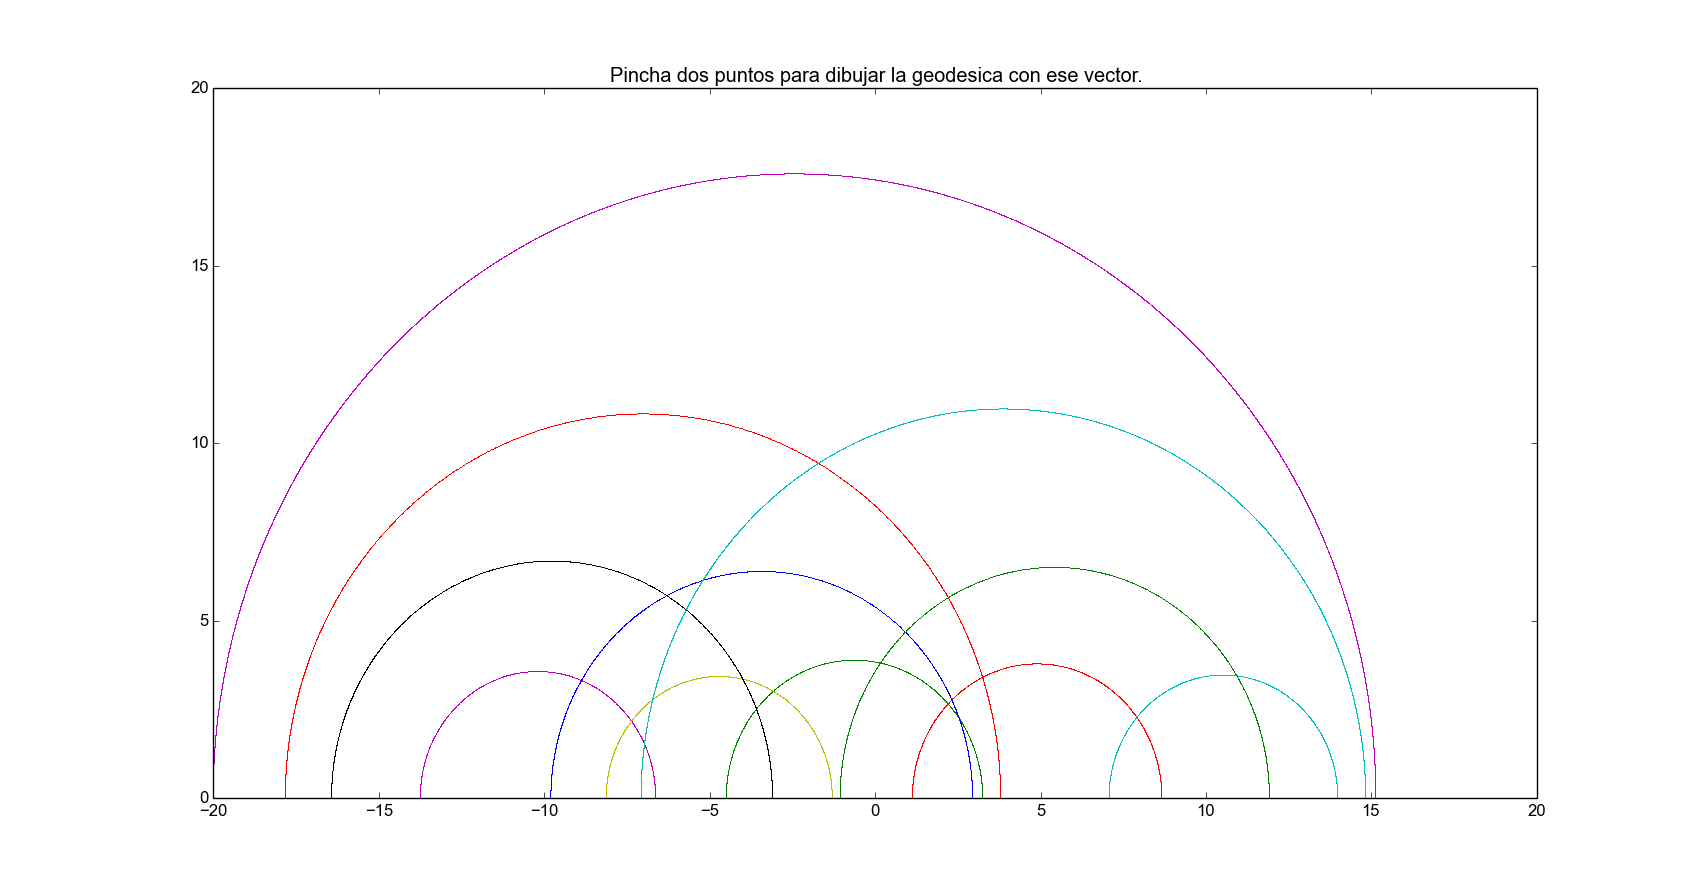
\includegraphics[width=0.8\textwidth]{./img/poincare.png}
  \end{center}
  \begin{itemize}
     \item Opcional:
       Partiremos del sistema de ecuaciones obtenido en clase:
       $$U''^{T} = \left[ \frac{1}{2}
        \left( \begin{array}{c}
           U'^{T}I_{u}U' \\
           U'^{T}I_{v}U'
           \end{array}\right)^{T}-U'^{T}\left(I_{u}u'+I_{v}v'\right)\right]I^{-1} $$\\ \\
 $$\left(u'' v''\right) = \left[ \frac{1}{2}
        \left(
           \left(u' v'\right)
           \left(\begin{array}{cc}
             0 & 0 \\ 
             0 & 0 
           \end{array}\right)
           \left(\begin{array} {c}
             u' \\
             v' 
           \end{array}\right)\ \ \ \left(u' v'\right)
           \left(\begin{array} {cc}
             \frac{-2}{v^{3}} & 0 \\ 
             0 &  \frac{-2}{v^{3}} 
           \end{array}\right)
           \left(\begin{array}{c}
             u' \\ 
             v' 
          
        \end{array} \right) \right)
           \ -
           \left(u' v'\right)
           \left(
           \left(\begin{array}{cc}
             0 & 0 \\ 
             0 & 0 
           \end{array}\right)u'
           +
           \left(\begin{array}{cc}
             \frac{-2}{v^{3}} & 0 \\ 
             0 & \frac{-2}{v^{3}} 
           \end{array}\right)v'\right)\right]
       \left(\begin{array}{cc} 
             v^{2} & 0 \\ 
             0 & v^{2} 
           \end{array}\right) $$\\ \\
       $$\left(u'' v''\right) =
       \left(\frac{2u'v'}{v}\ \ \frac{v'^2-u'^2}{v}\right)$$\ \
       %Resolviendo este problema con las condiciones iniciales:
       %$$ U(t_{0}) = U_{0} \ \ \ U'(t_{0}) = U'_{0}$$
       
       Tenemos, por tanto, las siguientes ecuaciones: \\
       \begin{equation}
         u''=2u'v'
       \end{equation}
       \begin{equation}
         v''=\frac{v'^2-u'^2}{v}
       \end{equation}

       Supongamos primero que $u'=0$. En este caso, la primera de las ecuaciones se satisface ($u''=0$) y las geodésicas tendrán la forma $u=cte$. \\

       Supongamos ahora que $u'\neq0$. Resolvemos para ello la segunda de las ecuaciones. Definimos $x=\frac{du}{dv}$. Así, $u'=xv'$. Derivando esta nueva ecuación mediante la regla de la cadena tenemos:
       \begin{equation}
         u''=\frac{dx}{dv}v'^2+xv''
       \end{equation}
       Sustituimos ahora (1) y (2) en la recién obtenida ecuación (3): \\
       \begin{equation*}
         \frac{2u'v'}{v}=\frac{dx}{dv}v'^2+x\frac{v'^2-u'^2}{v} 
       \end{equation*}
       Sustituimos el valor de $u'$ en la ecuación:
       \begin{equation*}
         \frac{dx}{dv}v'^2=\frac{2u'v'}{v}-x\frac{v'^2-x^2v'^2}{v}
       \end{equation*}
       Operando, tenemos finalmente:
       \begin{equation*}
         \frac{dx}{dv}=\frac{x+x^3}{v}
       \end{equation*}

       Despejando e integrando, sustituyendo la x por su valor ($u'/v'$) y volviendo a integrar, llegamos a la siguiente ecuación de la geodésica:
       \begin{equation*}
         (u-a)^2+v^2=(\frac{1}{b})^2
       \end{equation*}
       donde $a\in\mathbb{R}$, $b\in\mathbb{R}$ son constantes. Así, y teniendo en cuenta que $v>0$, las geodésicas serán semicírculos centrados en el punto $(a,0)$ y de radio $\frac{1}{b}$.
  \end{itemize}

\end{enumerate}
\end{document}
